\documentclass[bigger]{beamer}

\usepackage{pst-all} % PSTricks
\usepackage{tikz}
\usetikzlibrary{arrows,shapes,trees}
%--------------------------------------------------
% \usepackage{com.braju.pstricks} % The package that really does the hard work
% \usepackage{com.braju.graphicalmodels} % The package that really does the hard work
%-------------------------------------------------- 

\mode<presentation>{
  \usetheme{Pittsburgh}
  \usefonttheme{serif}
  \setbeamerfont{institute}{size=\normalsize}
  \setbeamerfont{section in toc}{size=\large}
  \setbeamerfont{subsection in toc}{size=\normalsize}
  \setbeamercovered{transparent}
  \setbeamertemplate{frametitle}{%
    \vskip 12pt
    \begin{centering}
    \structure{\textbf{\insertframetitle}}\par
    \end{centering}
  }
  \setbeamertemplate{footline}[page number]
}

\usepackage[english]{babel}
\usepackage{times}
\usepackage{algorithmic}
\usepackage{algorithm}
\usepackage{epsfig}
\usepackage{pgf}
\usepackage[absolute,overlay]{textpos}
%--------------------------------------------------
% \usepackage{mathtime}
%-------------------------------------------------- 

% Latin-1 only
\usepackage[latin1]{inputenc}
\usepackage[T1]{fontenc}
%--------------------------------------------------
% % Chinese-support
% \usepackage[nocjkbg5]{ucs}
% \usepackage[utf8x]{inputenc}
% \usepackage[C00,T1]{fontenc}
% \newcommand\tradtext[1]{\bgroup\fontencoding{C00}\fontfamily{ming}\selectfont%
% \SetUnicodeOption{cjkbg5}#1\egroup}
%-------------------------------------------------- 

\title[]{Relevance Model Revisited: With Multiple Document Representations}
\author[]{Ruey-Cheng Chen {\tt \scriptsize <cobain@turing.csie.ntu.edu.tw>}\\
Chiung-Min Tsai {\tt \scriptsize <cmtsai@mail.lis.ntu.edu.tw>}\\
Jieh Hsiang {\tt \scriptsize <jhsiang@ntu.edu.tw>}}
\institute{Dept. of Computer Science and Information Engineering\\
National Taiwan University, Taiwan}
\date[AIRS 2010]{AIRS 2010 (December 1, 2010)}
\subject{Information Retrieval}
%--------------------------------------------------
% \AtBeginSubsection[]
% {
%   \begin{frame}<beamer>
%     \frametitle{Outline}
%     \tableofcontents[currentsection,currentsubsection]
%   \end{frame}
% }
%-------------------------------------------------- 
%\beamerdefaultoverlayspecification{<+->}
\newcommand<>\ul[2]{\textbf{#1}\begin{itemize}#2\end{itemize} \vskip 0.5em}
\newcommand<>\ull[1]{\begin{itemize}#1\end{itemize}}
\newcommand<>\ol[2]{\textbf{#1}\begin{enumerate}#2\end{enumerate}}
\newcommand<>\oll[1]{\begin{enumerate}#1\end{enumerate}}
\newcommand<>\dl[2]{\textbf{#1}\begin{description}#2\end{description}}
\newcommand<>\f[2]{\begin{frame}{#1}#2\end{frame}}
\newcommand<>\mydef[2][]{\textbf{#1}\par#2\par}
\newcommand<>\tbl[3]{\textbf{#1}\vskip 0.5em\begin{center}\begin{tabular}{#2}#3\end{tabular}\end{center}}
\newcommand<>\fig[3]{\textbf{#1}\vskip 0.5em\begin{center}\begin{figure}\includegraphics[#2]{#3}\end{figure}\end{center}}
\newcommand<>\cols[1]{\begin{columns}#1\end{columns}}
\newcommand<>\col[2]{\begin{column}{#1}#2\end{column}}

\begin{document}

\frame{ \titlepage }

\f{Outline}{ \tableofcontents }

\section{Introduction}
\f{Homogeneity Assumption in IR}{
  
  Texts in a document is usually modeled as a set of terms, and every document
  possesses \textbf{only one} such representation

  \begin{itemize}
    \item Terms are assumed to be homogeneous \\
    (or drawn from a mixture of homogeneous sources)
    \item It leads to simple models
    \item It leaves no room for modeling heterogeneous data
  \end{itemize}
}

\f{Heterogeneous Data}{
  \begin{table}
    \centering
    \small
    \begin{tabular}{|l|l|}
      \hline
      Full-text & Long and loose textual content \\
      \hline
      Abstract & Summary of the content \\
      \hline
      Title & Short, conceptual description \\
      \hline
      Tags & Short, conceptual description (from the user side) \\
      \hline
      Metadata & Data describing the document \\
      \hline
    \end{tabular}
  \end{table}

  The data differ in scope, specificity, and semantics

  \begin{itemize}
    \item Under the homogeneity assumption, a document needs to be represented as a weighted combination
    \item Is there any other way out?
  \end{itemize}
}

\f{Idea: Layered Combination}{

  What if the model assumes \textit{multiple} document representations rather than only one?

  \begin{itemize}
    \item It is easy to incorporate heterogeneous data
    \item Retrieval can then be operated in different semantic layers
    \item Interoperability between layers is possible \\
    (and can be useful)
  \end{itemize}

  \vskip 1em
  Possible applications include

  \begin{itemize}
    \item Query expansion/refinement
    \item Facet ranking
  \end{itemize}
}

\f{Example: Articles and Authors}{
  \begin{table}
    \centering
    \footnotesize
    \begin{tabular}{l|p{6cm}|p{2cm}}
      & \textbf{Primary} (fulltext) & \textbf{Secondary} (author) \\
      \hline
      $\textrm{Article}_1$ & The sparsity which is implicit in MR images is exploited to significantly undersample
      k-space. Some MR images such as angiograms... & $\textrm{Author}_1$, $\textrm{Author}_4$ \\
      \hline
      $\textrm{Article}_2$ & Recently, a new direction in signal processing ``Compressed Sensing'' is being actively
      developed. A number of authors have pointed out... & $\textrm{Author}_2$, $\textrm{Author}_1$, $\textrm{Author}_3$ \\
      \hline
      $\ldots$ & $\ldots$ & $\ldots$
    \end{tabular}
  \end{table}

  \only<1>{
    Can we estimate this probability?
    \[ \Pr(\underbrace{\textrm{Author}_3}_\text{secondary term} | \underbrace{\textrm{``language modeling''}}_\text{primary term}) \]
  }
  \only<2>{
    Or, given a list of terminologies $T$, can we solve this?
    \[ t^* = \arg\max_{t \in T} \Pr(\underbrace{\textrm{Author}_3}_\text{secondary term} | \underbrace{t}_\text{primary term}) \]
  }
}

\f{Challenge: The Model}{

  Goal: To estimate the probability $\Pr(s|t)$, given that a document is indexed in
  two different vocabularies $T$ and $S$ (called the \emph{primary} and the
  \emph{secondary} term space, respectively)

  \vskip 1em
  Specifically, we want to estimate $\Pr(s|\mathbf{q})$ given the user query $\mathbf{q} \subset T$ 

  \begin{itemize}
    \item $\Pr(s|t)$ is the key to enable interactions
    \item It leads us to a generalization of the relevance model \cite{lavrenko2001relevance}
  \end{itemize}
}

\section{Related Work}

\f{Related Work}{
  Our method is inspired by the recent advances on language modeling
  \begin{itemize}
    \item Relevance model \cite{lavrenko2001relevance, zhai2001language}
    \item Bayesian language model \cite{zaragorza2003bayesian}
  \end{itemize}

  \vskip 1em
  Similar attempts toward facet ranking were made in the area of expert finding
  \begin{itemize}
    \item Inverse entity-frequency \cite{amitay2008finding}
    \item language-model-based approach \cite{balog2009language} 
  \end{itemize}
}

\f{Roadmap}{

  Our approach differs in:
  \begin{itemize}
    \item The presence of a secondary document representation
    \item The way document relevance is modeled 
    \item The way prior belief is supported
  \end{itemize}

  \vskip 1em
  Where do we go from here?
  \begin{itemize}
    \item We introduce an adaptation of the relevance model \cite{lavrenko2001relevance}
    (to cases where two representations are appropriate)
    \item We derive the model using Bayesian generative approach
    \item Two applications are introduced to evaluate our work 
  \end{itemize}
}

\section{Model}
\subsection{The Generative Framework}

\begin{frame}[fragile]
  \frametitle{The Generative Framework}
  \begin{figure}
    \centering
    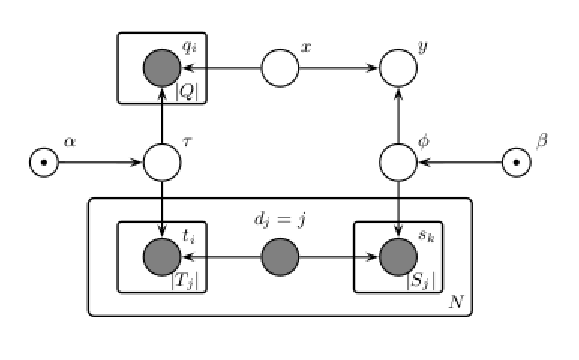
\includegraphics[width=8cm]{model}
  \end{figure}

  \begin{itemize}

    \only<1>{ \item Document $d_j$ is associated with two sets of terms $T_j$
    and $S_j$  \item Elements in $T_j$ and $S_j$ are drawn from two
    multinomials $\tau^{(j)}$ and $\phi^{(j)}$, respectively }
    
    \only<2>{ \item Two Dirichlets priors $\{\alpha_i; i \in [1, |T|]\}$ and
    $\{\beta_k; k \in [1, |S|]\}$ are assumed \item Some unknown document has
    generated $\mathbf{q}$ and $y$ }
    
  \end{itemize}

\end{frame}

\f{Generative Process}{
  For each document $d_j$:
  \begin{enumerate}
    \item $\tau^{(j)} \sim \textrm{Dirichlet}(\alpha_i; i \in [1, |T|])$
    \item $\phi^{(j)} \sim \textrm{Dirichlet}(\beta_k; k \in [1, |S|])$
    \item For $i \in \{ 1, \ldots, |T_j| \}$, $t_i \sim \textrm{Mult}(\tau^{(j)})$ 
    \item For $k \in \{ 1, \ldots, |S_j| \}$, $s_k \sim \textrm{Mult}(\phi^{(j)})$ 
  \end{enumerate}

  \vskip 1em
  \textbf{Goal}: Find $y^*$ by using the predictive distribution 
  \begin{equation} y^* = \arg\max_{y \in S} \Pr(y|\mathbf{q},
  \mathbf{t}, \mathbf{d}, \mathbf{s}) \label{eq:forward} \end{equation} 
  \begin{itemize}
    \item $\mathbf{t}$, $\mathbf{s}$, $\mathbf{d}$, $\mathbf{q}$: all the observed primary/secondary terms, documents, and query
  \end{itemize}
}

\subsection{Inference}

\f{Exact Inference}{
  Exact inference can be done with standard Bayesian approach
  \begin{eqnarray*}
    y^* &=& \arg\max_{y \in S} \sum_{x \in [1, N]} \Pr(y|x, \mathbf{q}, \mathbf{t}, \mathbf{d}, \mathbf{s}) \Pr(x|\mathbf{q}, \mathbf{t}, \mathbf{d}, \mathbf{s}) \nonumber\\
    \only<1>{
      &=& \arg\max_{y \in S} \sum_{x \in [1, N]} \left\{ \int \Pr(y|x, \phi^{(x)}) \Pr(\phi^{(x)}|d_x, \mathbf{s_x}) \mathrm{d}\phi^{(x)} \right. \nonumber\\
      && \left. \int \Pr(\mathbf{q}| x, \tau^{(x)}) \Pr(\tau^{(x)}|d_x, \mathbf{t_x})\mathrm{d}\tau^{(x)} \Pr(x) \right\} \nonumber\\
    }
    \only<2>{
      &=& \arg\max_{y \in S} \sum_{x \in [1, N]} \frac{\beta_y + c_{y,x}}{\sum_k \beta_k + c_{k,x}} \frac{\mathcal{B}(\{\alpha_i + c_{i,x} + c_{i,q}; \forall i \})}{\mathcal{B}(\{\alpha_i + c_{i,x} ; \forall i\})} \Pr(x) \nonumber
    }
  \end{eqnarray*}

  \begin{itemize}
  \only<1>{
    \item $\mathbf{t_x}, \mathbf{s_x}$: All the primary/secondary terms of $d_x$
    \item $\phi^{(x)}, \tau^{(x)}$: The primary/secondary multinomials of $d_x$
  }
  \only<2>{
    \item $c_{k,x}, c_{k,q}$: The counts of term $k$ in document $x$/query $\mathbf{q}$
    \item $\mathcal{B}(\cdot)$: The multinomial beta
    function\\
    i.e., $\mathcal{B}(a_1, \ldots, a_n) = (\prod_i
    \Gamma(a_i)) / \Gamma(\sum_i a_i)$
  }
  \end{itemize}
}

\f{Implication}{

  The equation can be interpreted as an expectation of a weighted sum
  \[ \sum_{x \in [1, N]} \overbrace{\frac{\beta_y + c_{y,x}}{\sum_k \beta_k +
  c_{k,x}}}^\text{normalized count} \overbrace{\frac{\mathcal{B}(\{\alpha_i +
  c_{i,x} + c_{i,q}; \forall i \})}{\mathcal{B}(\{\alpha_i + c_{i,x} ;
  \forall i\})}}^\text{relevance} \Pr(x) \]

  \begin{itemize}
    \item Normalize the count of term $y$
    \item Weight the normalized count by the document relevance 
    \item The expectation can be achieved without knowing $x$
  \end{itemize}

}

\subsection{Hyperparameters and the Index Structure}

\f{Priors}{

  Uniform prior
  \begin{itemize}
    \item $U(c) = (c, c, \ldots, c)$
    \item Parametrized by some constant $c$
  \end{itemize}
  
  \vskip1em
  Smoothed-Dirichlet prior
  \begin{itemize}
    \item $D(\mu) = (\mu \Pr(w_1), \mu \Pr(w_2), \ldots, \mu \Pr(w_n))$ 
    \item $\Pr(w_k)$: the probability of generating term $w_k$ (from either term space) from the collection 
    \item Parametrized by some constant $\mu$
    \item Widely-used smoothing method in IR \cite{zhai2004study}
  \end{itemize}
}

\f{Language Model Integration}{

  Given $\alpha = D(\mu)$ and $\Pr(x) = U(c)$, we have

  \[ \Pr(y|\mathbf{q}, \mathbf{t}, \mathbf{d}, \mathbf{s}) \propto
  \sum_{x \in [1, N]} \frac{\beta_y + c_{y,x}}{\sum_k \beta_k + c_{k,x}}
  {\rm L}_{\rm LM}(\mathbf{q}|x) \]

  \begin{itemize}

    \item ${\rm L}_{\rm LM}(\mathbf{q}|x)$: The query likelihood score by using
    language model with Dirichlet smoothing

    \item It can be shown that document relevance is proportional to ${\rm
    L}_{\rm LM}(\mathbf{q}|x)$ in this special case

    \item Efficient computation is possible with a forward index over the
    secondary terms

  \end{itemize}
}

\section{Experimental Results}
\subsection{Query Refinement Using the Secondary Representation}

\f{Query Refinement Using the Secondary Representation}{
  \begin{figure}
    \centering
    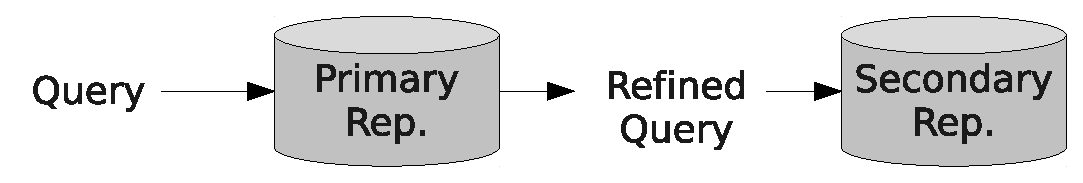
\includegraphics[width=8cm]{qr}
  \end{figure}

  Idea: A two-stage retrieval approach
  \begin{itemize}
    \item Make an initial run over all the terms (primary)
    \item Make a second run over only highly-discriminative terms (secondary)
    \item Use the estimate $\Pr(y|\mathbf{q}, \mathbf{t}, \mathbf{d}, \mathbf{s})$ as the refined query
  \end{itemize}
}

\f{Evaluation Setup}{
  Chinese-to-Chinese monolingual document retrieval, NTCIR-4 CLIR Task
  \begin{itemize}
    \item 381,681 newswire articles, 59 test topics, title queries only
    \item Primary: CJK-character bigrams + English word unigrams
    \item Secondary: Top-500,000 high discriminative CJK-character bigrams \\
      (ranked by tf-idf, with min. support 5)
  \end{itemize}

  \vskip 1em
  Baseline
  \begin{itemize}
    \item tfidf/okapi + pseudo relevance feedback
    \item indri + relevance model
    \item The number of feedback documents/terms: 20/100
  \end{itemize}
}

\f{Evaluation Result}{
  \begin{table}
    \scriptsize
    \centering
    \begin{tabular}{lllllllll}
      & \multicolumn{4}{c}{Rigid Judgment} & \multicolumn{4}{c}{Relax Judgment} \\
      \hline
      Regular & MAP & (+\%) & P@5 & (+\%) & MAP & (+\%) & P@5 & (+\%) \\
      \hline
      {\tt tfidf} & 0.181 & & 0.264 & & 0.213 & & 0.335 & \\
      {\tt okapi} & 0.185 & & 0.278 & & 0.223 & & 0.356 & \\
      {\tt indri} & 0.174 & & 0.258 & & 0.216 & & 0.346 & \\
      {\tt lm}    & 0.170 & & 0.251 & & 0.209 & & 0.322 & \\
      \hline
      Expansion & & & & & & & & \\
      \hline
      {\tt tfidf+PRF} & 0.217 & (+20\%) & 0.295 & (+12\%) & 0.264 & (+24\%) & 0.383 & (+14\%) \\
      {\tt okapi+PRF} & \textbf<1>{0.224} & (+21\%) & \textbf<1>{0.315} & (+13\%) & \textbf<1>{0.270} & (+21\%) & \textbf<1>{0.400} & (+12\%) \\
      {\tt indri+RM} & 0.180 & (+3\%) & 0.271 & (+5\%) & 0.222 & (+3\%) & 0.342 & (-1\%) \\
      {\tt lm+BRM} & \textbf<2>{0.207} & (+22\%) & \textbf<2>{0.302} & (+20\%) & \textbf<2>{0.261} & (+25\%) & \textbf<2>{0.369} & (+15\%)
    \end{tabular}
  \end{table}

  \begin{itemize}
    \only<1>{
      \item The overall best run is {\tt okapi+PRF}
      \item Performance gap between tfidf-based and LM-based methods remains large 
    }
    \only<2>{
      \item {\tt lm+BRM} outperforms {\tt indri+RM} by 17.6\% in MAP
      \item {\tt lm+BRM} shows roughly comparable performance against that of {\tt tfidf+PRF}
    }
  \end{itemize}
}

\f{Analysis}{
  The performance results on the top-500k bigram representation only
  \begin{table}
    \scriptsize
    \centering
    \begin{tabular}{p{3cm}p{1.5cm}p{1.5cm}p{1.5cm}l}
      & \multicolumn{2}{c}{Rigid Judgment} & \multicolumn{2}{c}{Relax Judgment} \\
      \hline
      Method & MAP & P@5 & MAP & P@5 \\
      \hline
      {\tt tfidf+PRF.500k} & 0.190 & 0.288 & 0.241 & 0.373 \\
      {\tt okapi+PRF.500k} & 0.196 & {\bf 0.302} & 0.247 & {\bf 0.383} \\
      {\tt indri+RM.500k} & 0.155 & 0.248 & 0.197 & 0.309 \\
      \multicolumn{5}{c}{({\it The above runs were indexed against top-500k bigrams only})} \\
      \hline
      {\tt lm+BRM} & {\bf 0.207} & {\bf 0.302} & {\bf 0.261} & 0.369 \\
      \multicolumn{5}{c}{({\it This run was operated on both representations})}
    \end{tabular}
  \end{table}

  \begin{itemize}
    \item It leads to degraded performance
    \item It favors our first-recall-then-precision idea 
    \item Question: Can layered approach also be applied to tfidf-based methods?
  \end{itemize}
}

\subsection{Retrieving Query-Relevant Facets}

\f{Retrieving Query-Relevant Facets}{

  In faceted search \cite{hearst2002finding,yee2003faceted,roy2008minimum},
  facets are usually sorted in descending order of the number of counts
  \begin{itemize}
    \item Easy to implement (one pass through the forward index)
    \item Critics \#1: It disregards the notion of relevance

    \item Critics \#2: Users can be mislead when consulting the results to
    guide the subsequent exploratory search

  \end{itemize}

  \vskip 1em Idea: Encode facets into the secondary representation and sort
  them by using $\Pr(y|\mathbf{q}, \mathbf{t}, \mathbf{d}, \mathbf{s})$

}

\f{Evaluation Setup}{
  Benchmark: Retrieving relevant facets on Tan-Hsin Corpus
  \begin{itemize}
    \item 15,314 historical documents, each with person name facets
    \item Using 28 randomly-selected topics \\
    (out of 105 query topics collected from query logs)
    \item Relevance judgment was manually made on the top-100 facets returned
  \end{itemize}

  \vskip 1em
  Participating runs include
  \begin{itemize}
    \item The count-based scheme (baseline)
    \item The proposed method, using uniform prior for $\beta$
    \item The proposed method, using smoothed Dirichlet prior for $\beta$ 
  \end{itemize}
}

\f{Evaluation Result}{
  \begin{table}
    \scriptsize
    \centering
    \begin{tabular}{llll}
      Method & & MAP & P@10 \\
      \hline
      {\tt baseline} & & 0.2996 & 0.3857 \\
      {\tt uniform-prior} & $\beta = 0$ & 0.5775 & 0.6179\\
      & $\beta = 1$ & \textbf{0.5899} & \textbf{0.6464} \\
      & $\beta = 10$ & 0.5877 & \textbf{0.6464} \\
      {\tt smoothed-prior} & $\mu = 0.01$ & 0.5781 & 0.6179 \\
      & $\mu = 1$ & 0.5782 & 0.6214 \\
      & $\mu = 100$ & 0.4956 & 0.5429 \\
    \end{tabular}
  \end{table}

  \begin{itemize}
    \item Proposed methods demote less informative facets 

    \item Proposed methods outperform the baseline\\
    (ranging from 30\% to 100\% in MAP)

    \item Our model achieved comparable performance against LM-based method
    \cite{balog2009language} (roughly a special case of {\tt uniform-prior}
    with $\beta = 0$)

    \item {\tt smoothed-prior} suffers from data sparsity
  \end{itemize}
}

\section{Discussion and Concluding Remarks}
\f{Concluding Remarks}{
  Our proposed framework:
  \begin{itemize}
    \item Offers interoperability between two different term domains
    \item Achieves satisfactory results in both applications
    \item Serves as a stepping stone to explore the use of multiple document representations in IR
  \end{itemize}

  \vskip 1em
  We are currently looking at these issues
  \begin{itemize}
    \item Can topic-biased priors be useful?
    \item How do we generalize the first-recall-then-precision method?
    \item How do we deal with data sparsity in facet ranking?
  \end{itemize}
}

\section<presentation>*{\appendixname}

\frame{
  \begin{center}
    \Huge{Thanks for your attention!}
    \par
    Any Question?
  \end{center}
}

\begin{frame}[allowframebreaks]
  \frametitle{References}
  \small
  \bibliography{slides}
  \bibliographystyle{apalike}
\end{frame}

\f{Inference (For Impatient Readers)}{
  \begin{eqnarray}
    && \Pr(y|\mathbf{q}, \mathbf{t}, \mathbf{d}, \mathbf{s})
    = \sum_{x \in [1, N]} \Pr(y|x, \mathbf{q}, \mathbf{t}, \mathbf{d}, \mathbf{s}) \Pr(x|\mathbf{q}, \mathbf{t}, \mathbf{d}, \mathbf{s}) \nonumber\\
    &\propto& \sum_{x \in [1, N]} \left\{ \int \Pr(y|x, \phi^{(x)}) \Pr(\phi^{(x)}|d_x, \mathbf{s_x}) \mathrm{d}\phi^{(x)} \right. \nonumber\\
    && \left. \int \Pr(\mathbf{q}| x, \tau^{(x)}) \Pr(\tau^{(x)}|d_x, \mathbf{t_x})\mathrm{d}\tau^{(x)} \Pr(x) \right\} \nonumber\\
    &=& \alert{\sum_{x \in [1, N]} \frac{\beta_y + c_{y,x}}{\sum_k \beta_k + c_{k,x}} \frac{\mathcal{B}(\{\alpha_i + c_{i,x} + c_{i,q} \})}{\mathcal{B}(\{\alpha_i + c_{i,x} \})} \Pr(x)} \label{eq:forward-solution}
  \end{eqnarray}
  \begin{itemize}
    \item $\mathcal{B}(\cdot)$ is the multinomial beta
    function defined by $\mathcal{B}(a_1, \ldots, a_n) = (\prod_i
    \Gamma(a_i)) / \Gamma(\sum_i a_i)$
  \end{itemize}
}

\f{Inference: Step by Step}{
  Inducing the first term in the summation
  \begin{eqnarray*}
    \Pr(y|\mathbf{q}, \mathbf{t}, \mathbf{d}, \mathbf{s}) &=& \sum_{x \in
    [1, N]} \alert{\Pr(y|x, \mathbf{q}, \mathbf{t}, \mathbf{d}, \mathbf{s})}
    \Pr(x|\mathbf{q}, \mathbf{t}, \mathbf{d}, \mathbf{s}) \nonumber\\
    && \nonumber\\
    \Pr(y|x, \mathbf{q}, \mathbf{t}, \mathbf{d}, \mathbf{s})
    &=& \int \Pr(y, \phi^{(x)}|x, \mathbf{q}, \mathbf{t}, \mathbf{d}, \mathbf{s}) \mathrm{d}\phi^{(x)} \nonumber\\
    &=& \int \Pr(y|\phi^{(x)}, x, \mathbf{q}, \mathbf{t}, \mathbf{d}, \mathbf{s}) 
    \Pr(\phi^{(x)}|x, \mathbf{q}, \mathbf{t}, \mathbf{d}, \mathbf{s}) \mathrm{d}\phi^{(x)} \nonumber\\
    &=& \int \Pr(y|\phi^{(x)}, x) \Pr(\phi^{(x)}|d_x, \mathbf{s}_x) \mathrm{d}\phi^{(x)} \label{eq:first}
  \end{eqnarray*}
}

\f{Inference: Step by Step}{
  Inducing the second term in the summation
  \begin{eqnarray*}
    \Pr(y|\mathbf{q}, \mathbf{t}, \mathbf{d}, \mathbf{s}) &=& \sum_{x \in
    [1, N]} \Pr(y|x, \mathbf{q}, \mathbf{t}, \mathbf{d}, \mathbf{s})
    \alert{\Pr(x|\mathbf{q}, \mathbf{t}, \mathbf{d}, \mathbf{s})} \nonumber\\
    && \nonumber\\
    \Pr(x|\mathbf{q}, \mathbf{t}, \mathbf{d}, \mathbf{s})
%--------------------------------------------------
%     &=& \frac{\Pr(\mathbf{q}|x, \mathbf{t}, \mathbf{d}, \mathbf{s}) \Pr(x|\mathbf{t}, \mathbf{d}, \mathbf{s})}
%     {\Pr(\mathbf{q}|\mathbf{t}, \mathbf{d}, \mathbf{s})} \nonumber\\
%-------------------------------------------------- 
    &\propto& \Pr(\mathbf{q}|x, \mathbf{t}, \mathbf{d}, \mathbf{s}) \Pr(x|\mathbf{t}, \mathbf{d}, \mathbf{s}) \nonumber\\
    &=& \left( \int \Pr(\mathbf{q}, \tau^{(x)}|x, \mathbf{t}, \mathbf{d}, \mathbf{s}) \mathrm{d}\tau^{(x)} \right) 
    \Pr(x|\mathbf{t}, \mathbf{d}, \mathbf{s}) \nonumber\\
    &=& \left( \int \Pr(\mathbf{q}|\tau^{(x)}, x, \mathbf{t}, \mathbf{d}, \mathbf{s}) 
    \Pr(\tau^{(x)}|x, \mathbf{t}, \mathbf{d}, \mathbf{s}) \mathrm{d}\tau^{(x)} \right) \nonumber\\
    && \Pr(x|\mathbf{t}, \mathbf{d}, \mathbf{s}) \nonumber\\
    &=& \int \Pr(\mathbf{q}|\tau^{(x)}, x) \Pr(\tau^{(x)}|d_x, \mathbf{t}_x) \mathrm{d}\tau^{(x)} \Pr(x) \label{eq:second}
  \end{eqnarray*}
}

\f{Inference: Conjugate Priors}{
  In Bayesian theory, the prior $\Pr(\theta)$ and posterior $\Pr(\theta|x)$
  are called conjugate distributions, if the posterior are in the same family as the prior
  \begin{itemize}
    \item Viewed as updating the prior belief on
    $\theta$ after observing a sequence of outcome $x$
    \item Algebraically ``syntactic sugar'' to simplify inference
  \end{itemize}

  \vskip 1em
  Fast fact: Dirichlets are conjugate to multinomials (see Gelman et al.)
  \begin{itemize}
    \item $\Pr(\phi^{(x)}|x, y, d_x, \mathbf{s}_x) \sim \mathrm{Dirichlet}(\{\beta_k + c_{k,x}; \forall k\})$
    \item $\Pr(\tau^{(x)}|x, \mathbf{q}, d_x, \mathbf{t}_x) \sim \mathrm{Dirichlet}(\{\alpha_i + c_{i,x} + c_{i,q}; \forall i\})$
  \end{itemize}
}

\f{Inference: Revisited}{
  Now, integrating out the priors
  \begin{eqnarray*}
  \int \Pr(y|x, \phi^{(x)}) \Pr(\phi^{(x)}|d_x, \mathbf{s_x}) \mathrm{d}\phi^{(x)} 
  &=& \frac{\beta_y + c_{y,x}}{\sum_k \beta_k + c_{k,x}} \\
  \int \Pr(\mathbf{q}| x, \tau^{(x)}) \Pr(\tau^{(x)}|d_x, \mathbf{t_x})\mathrm{d}\tau^{(x)} 
  &=& \frac{\mathcal{B}(\{\alpha_i + c_{i,x} + c_{i,q} \})}{\mathcal{B}(\{\alpha_i + c_{i,x} \})} 
  \end{eqnarray*}

  \vskip 1em
  We obtain the closed-form solution
  \begin{eqnarray*}
    \Pr(y|\mathbf{q}, \mathbf{t}, \mathbf{d}, \mathbf{s}) 
    &=& \sum_{x \in [1, N]} \Pr(y|x, \mathbf{q}, \mathbf{t}, \mathbf{d}, \mathbf{s}) \Pr(x|\mathbf{q}, \mathbf{t}, \mathbf{d}, \mathbf{s}) \nonumber\\
    &\propto& \alert{\sum_{x \in [1, N]} \frac{\beta_y + c_{y,x}}{\sum_k \beta_k + c_{k,x}} \frac{\mathcal{B}(\{\alpha_i + c_{i,x} + c_{i,q} \})}{\mathcal{B}(\{\alpha_i + c_{i,x} \})} \Pr(x)}
  \end{eqnarray*}
}

\f{Query Refinement Using the Secondary Representation}{
  Facilitating the second-run retrieval
  \begin{itemize}
    \item The refined model is a probability distribution
    \item For each $s_k$, we calculated its \emph{expectation} $E(s_k|\mathbf{q}, \mathbf{t}, \mathbf{d}, \mathbf{s})$
    \item The expectation can be seen as the number of occurrence for $s_k$
    \item The resulting language model is: \[
      x^{*} = \arg\max_x \prod_k \Pr(s_k|x)^{E(s_k|\mathbf{q}, \mathbf{t}, \mathbf{d}, \mathbf{s})}
    \]
    \item This simple technique reduces to KL-divergence retrieval framework \cite{zhai2001language}
  \end{itemize}
}


\end{document}
